\documentclass[paper=a4, fontsize=12pt]{scrartcl}

\usepackage{graphicx}
\usepackage{siunitx}
\usepackage{amsmath}
\usepackage{mathrsfs}
\usepackage{float}
\usepackage{subfig}
\graphicspath{{./img/}}

\title{
	\normalfont \normalsize
	\textsc{University of Ottawa} \\ [5pt]
	\huge Discrete-Velocity Scheme Project
}
\author{Mathieu Marchildon} % Your name
\date{\normalsize \today} % Today's date or a custom date


\begin{document}
\maketitle


\section*{Shock-Tube Problem}
For the initial conditions of the shock-tube we must select an appropriate velocity space.
This velocity space can be determined by observing the distribution function on each side of
the shock tube for both initial conditions.
The distribution function in velocity space can be determined by applying Maxwell-Boltzmann distribution
for various ranges in velocity space.
\[
        f = \frac{\rho}{m} \Big( \frac{\rho}{2 \pi p}\Big)^{\frac{1}{2}}e^{\frac{\rho}{2 p}c^2}
\]



\begin{figure}[H]%
    \centering
    \subfloat[Left inital conditions]{{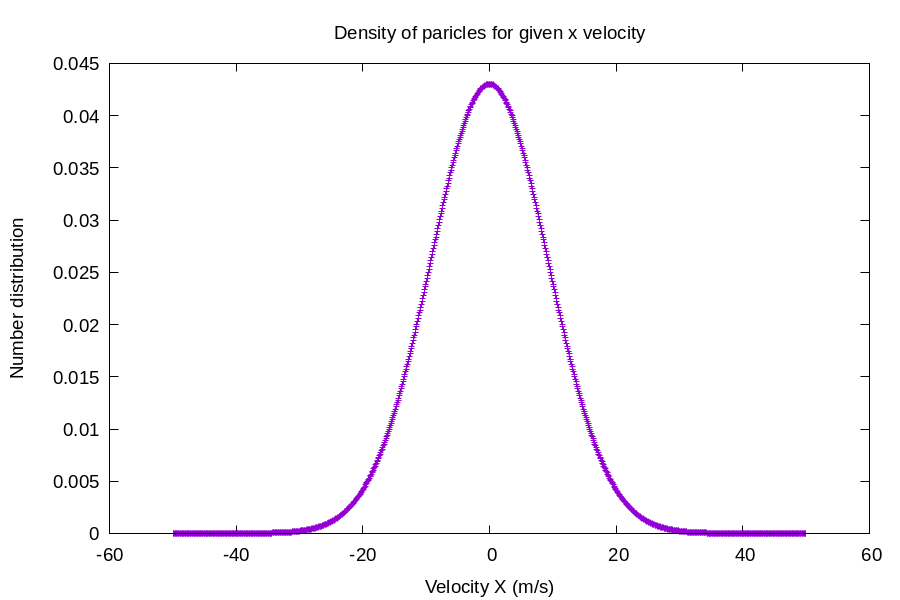
\includegraphics[width=7cm]{left_init_50} }}%
    \qquad
    \subfloat[Right inital conditions]{{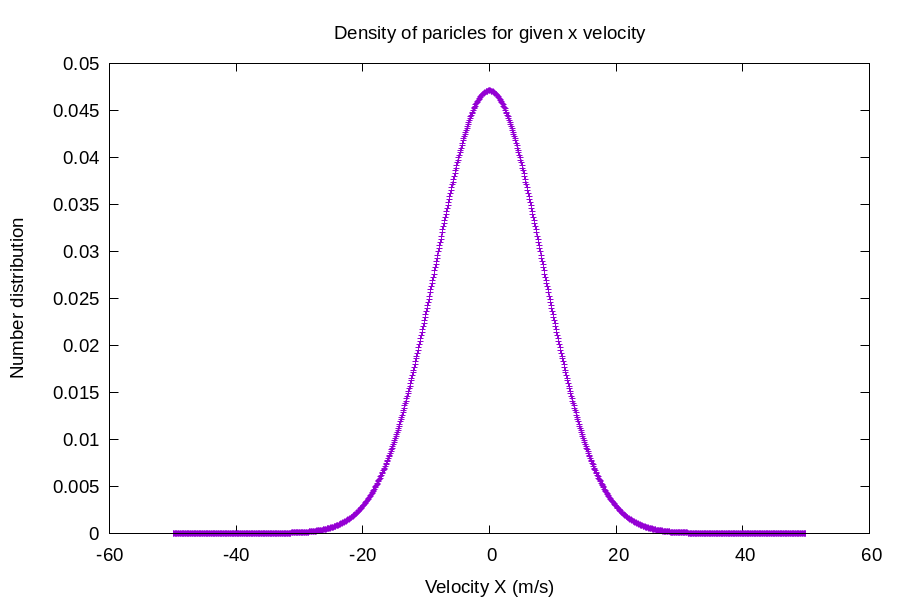
\includegraphics[width=7cm]{right_init_50} }}%
    \caption{Distribution function at initial conditions \newline velocity range of $\pm \SI{50}{\meter \per \second}$
 }
    \label{fig:init_50}%
\end{figure}
Figure \ref{fig:init_50} shows the distribution function for the left and right initial conditions.
The velocity space selected was ranging from $\SI{-50}{\meter \per \second}$ to $\SI{50}{\meter \per \second}$
This range of velocity seem way too large as the number density is near zero at the $\SI{30}{\meter \per \second}$
range
\begin{figure}[H]%
    \centering
    \subfloat[Left inital conditions]{{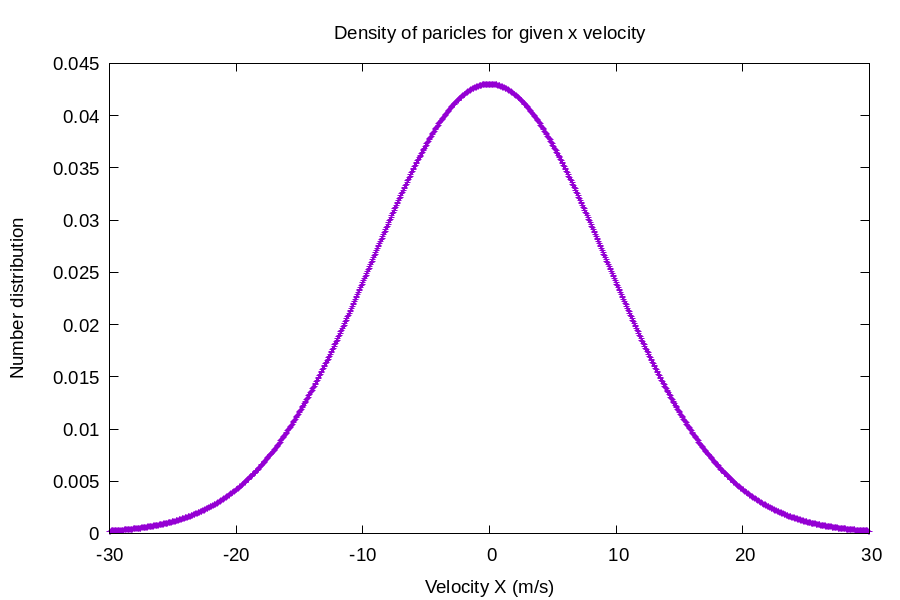
\includegraphics[width=7cm]{left_init_30} }}%
    \qquad
    \subfloat[Right inital conditions]{{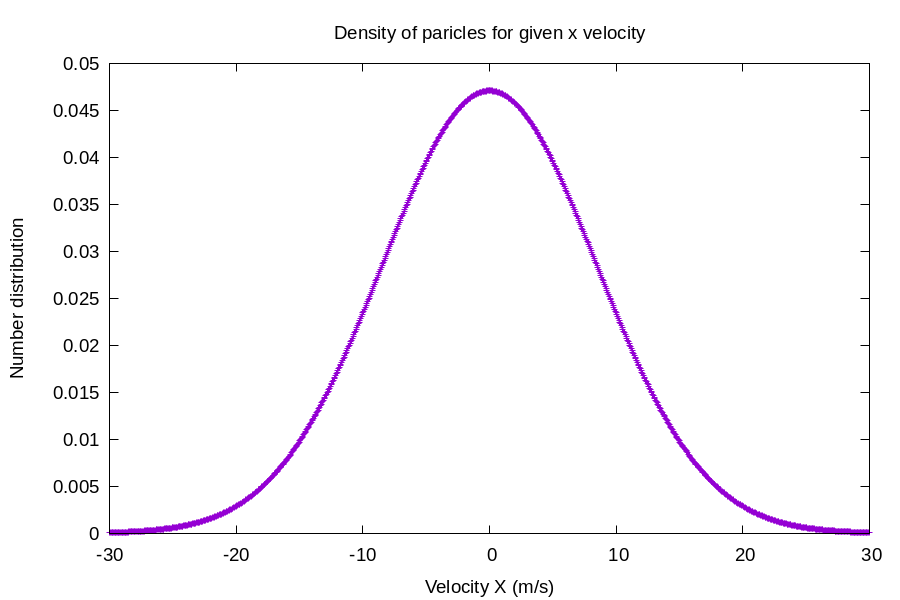
\includegraphics[width=7cm]{right_init_30} }}%
    \caption{Distribution function at initial conditions \newline velocity range of $\pm \SI{30}{\meter \per \second}$
 }
    \label{fig:init_30}%
\end{figure}
Selecting a velocity range of $\pm \SI{30}{\meter \per \second}$, as shown in \ref{fig:init_30} we obtain
a more refined velocity space.
Such that we are not computing properties of particles who's number density is near zero.


\end{document}
